\documentclass[letterpaper,11pt]{article}
\oddsidemargin -1.0cm \textwidth 17.4cm

\usepackage[utf8]{inputenc}
\usepackage[activeacute,spanish]{babel}
\usepackage{amsfonts,setspace}
\usepackage{amsmath}
\usepackage{amssymb, amsmath, amsthm}
\usepackage{comment}
\usepackage{amssymb}
\usepackage{dsfont}
\usepackage{anysize}
\usepackage{multicol}
\usepackage{enumerate}
\usepackage{graphicx}
\usepackage[left=2cm,top=2cm,right=2cm, bottom=2cm]{geometry}
\setlength\headheight{2em} 
\usepackage{fancyhdr}
\usepackage{multicol}
\pagestyle{fancy}
\fancyhf{}


\renewcommand{\labelenumi}{\normalsize\bfseries P\arabic{enumi}.}
\renewcommand{\labelenumii}{\normalsize\bfseries (\alph{enumii})}
\renewcommand{\labelenumiii}{\normalsize\bfseries \roman{enumiii})}


\DeclareMathOperator{\sen}{sen}
\DeclareMathOperator{\senh}{senh}
\DeclareMathOperator{\arcsen}{arcsen}
\DeclareMathOperator{\tg}{tg}
\DeclareMathOperator{\arctg}{arctg}
\DeclareMathOperator{\ctg}{ctg}
\DeclareMathOperator{\dom}{Dom}
\DeclareMathOperator{\sech}{sech}
\DeclareMathOperator{\rec}{Rec}
\DeclareMathOperator{\inte}{Int}
\DeclareMathOperator{\adh}{Adh}
\DeclareMathOperator{\fr}{Fr}
\DeclareMathOperator{\Ima}{Im}
\DeclareMathOperator{\dist}{dist}
\DeclareMathOperator{\argmin}{\text{argmín}}
\let\lim=\undefined\DeclareMathOperator*{\lim}{\text{lím}}
\let\max=\undefined\DeclareMathOperator*{\max}{\text{máx}}
\let\min=\undefined\DeclareMathOperator*{\min}{\text{mín}}
\let\inf=\undefined\DeclareMathOperator*{\inf}{\text{ínf}}


\newcommand{\pint}[2]{\left< #1,#2\right>}
\newcommand{\ssi}{\Longleftrightarrow}
\newcommand{\conv}[2]{\xrightarrow[#1\to#2]{}}
\newcommand{\imp}{\Longrightarrow}
\newcommand{\pmi}{\Longleftarrow}
\newcommand{\ipartial}[2]{\dfrac{\partial #1}{\partial #2}}
\newcommand{\ider}[2]{\dfrac{d #1}{d #2}}
\newcommand{\iipartial}[2]{\dfrac{\partial^2 #1}{\partial #2^2}}
\newcommand{\iider}[2]{\dfrac{d^2 #1}{d #2^2}}
\newcommand{\ijpartial}[3]{\dfrac{\partial^2 #1}{\partial #2 \partial #3}}
\newcommand{\N}{\mathbb{N}}
\newcommand{\Z}{\mathbb{Z}}
\newcommand{\C}{\mathbb{C}}
\newcommand{\Q}{\mathbb{Q}}
\newcommand{\R}{\mathbb{R}}
\newcommand{\K}{\mathbb{K}}
\newcommand{\sol}{\textbf{\emph{Soluci\'on: }}}
\newcommand{\dem}{\textbf{\emph{Demostraci\'on: }}}
\newcommand{\aux}[4]{\Large \textbf{Clase Auxiliar N#1: #2}}
\newcommand{\pauta}[4]{\Large \textbf{Pauta #1 N#2}}
\newcommand{\enc}[3]{\Large \textbf{#1}}
\newcommand{\norm}[1]{\lVert #1\rVert }
\newcommand{\vabs}[1]{\lvert #1\rvert}

\begin{document}

\fancyhead[L]{\itshape{Facultad de Ciencias F\'isicas y Matem\'aticas}}
\fancyhead[R]{\itshape{Universidad de Chile}}

\begin{minipage}{11.5 cm}
\begin{flushleft}
\hspace*{-0.6cm}\textbf{MA2001-4 Cálculo en Varias Variables}\\
\hspace*{-0.6cm}\textbf{Profesor:} Javier Ramírez G.\\
\hspace*{-0.6cm}\textbf{Auxiliar:} Alejandro Silva C.\\

\end{flushleft}
\end{minipage}

\begin{picture}(2,3)
    \put(370,-4){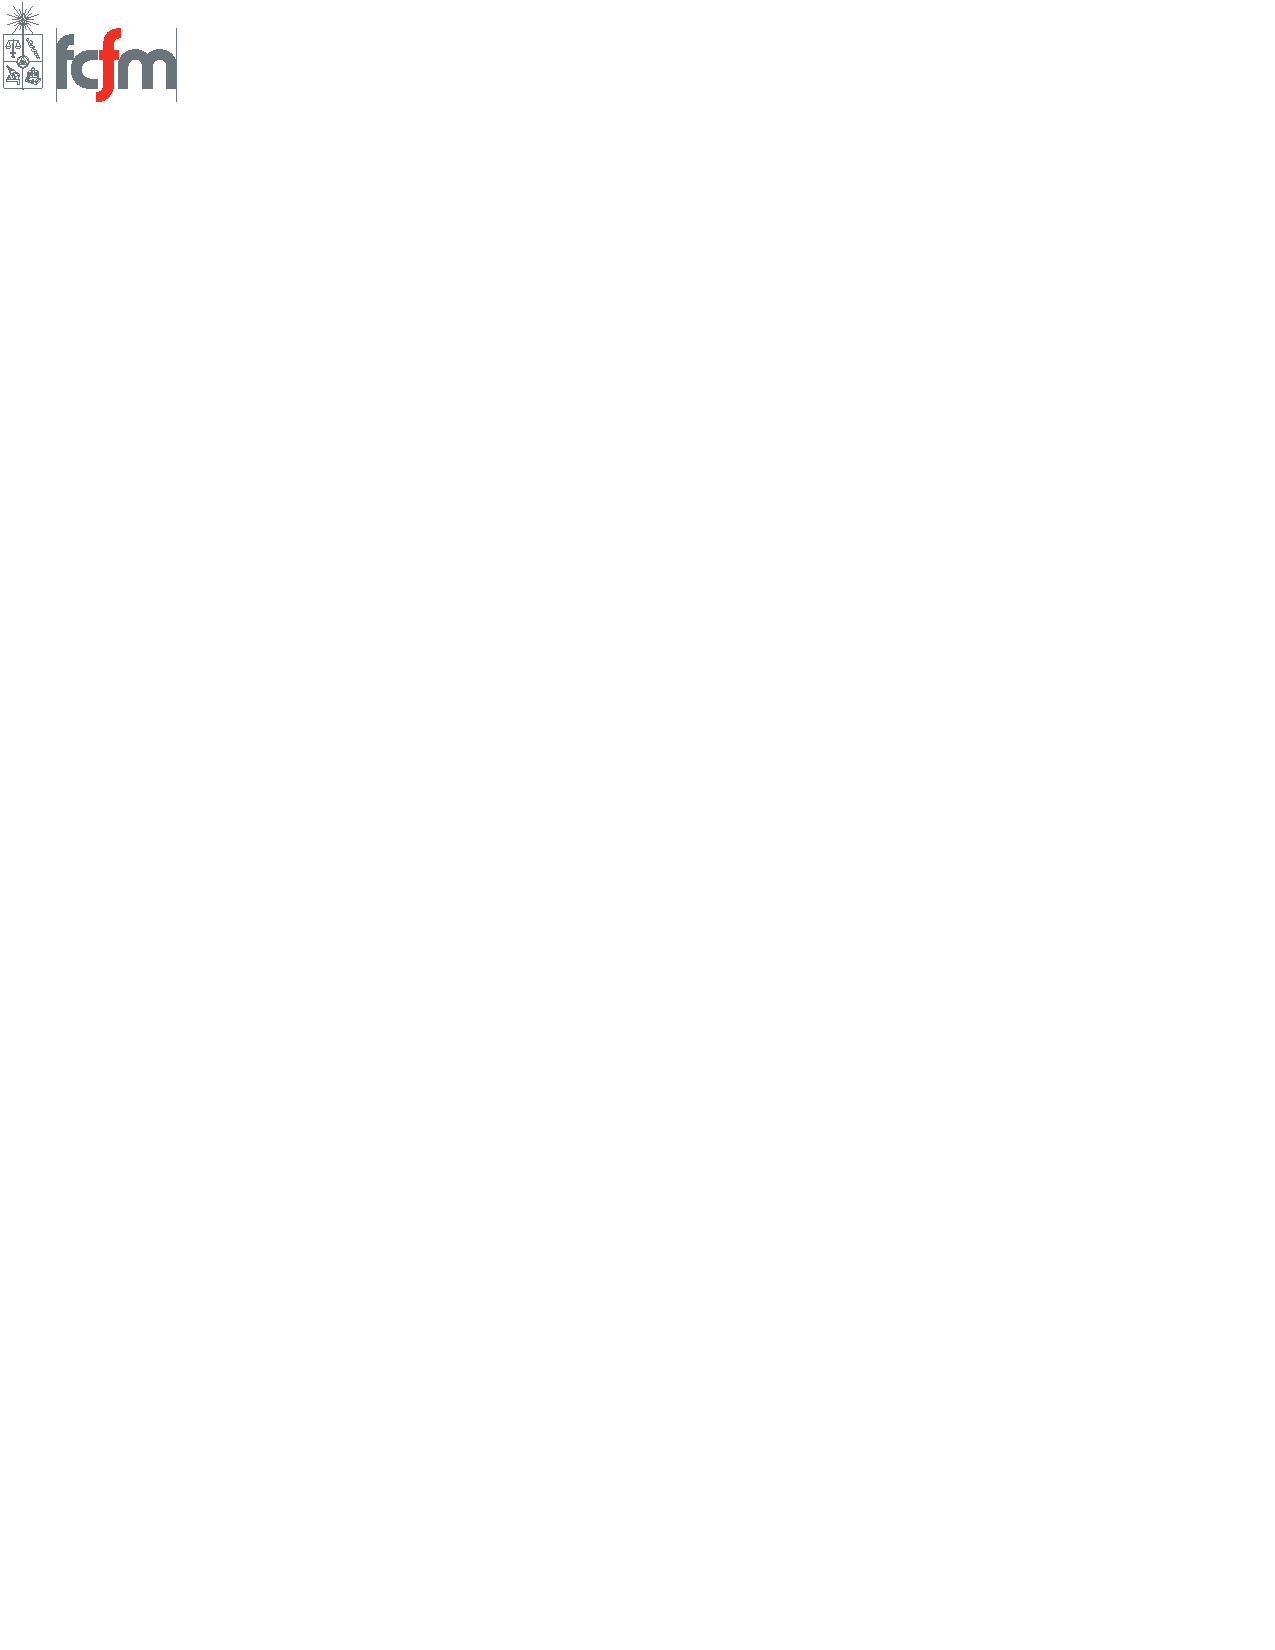
\includegraphics[scale=1.2]{fcfm2.pdf}}
\end{picture}

\begin{center}
	\LARGE \bf{Pauta auxiliar \#5}\\
\end{center}

\vspace{-1cm}
\begin{enumerate}\setlength{\itemsep}{0.4cm}	
\item[]
\end{enumerate}
\begin{enumerate}
\item En esta pregunta probaremos el siguiente resultado de gran utilidad:\\

\textit{\underline{\textbf{Prop:}} Sea $\Omega \subseteq E, f:E\to F$ y $x_0 \in \text{acc}(\Omega)\cap \Omega$, entonces
\[f \text{ es continua en } x_0 \ssi \forall\,(x_n)_{n\in\N}\subseteq\Omega\setminus\{x_0\}, x_n\conv{n}{\infty}x_0 \imp f(x_n)\conv{n}{\infty}f(x_0).\]
}
Esto quiere decir que para probar la continuidad de una función en un punto de acumulación, no es necesario considerar los casos en que la sucesión pasa por el punto.

\dem Recordemos primero las definiciones que ocuparemos:
\begin{itemize}
    \item[\textbf{Def:}] Sea $\Omega\subseteq E$ y $x\in E$ (no necesariamente en $\Omega$). Decimos que $x$ es \textbf{punto de acumulación} de $\Omega$ si $x\in\adh(\Omega\setminus\{x\})$
    \item[\textbf{Def:}] Sea $\Omega \subseteq E, f:E\to F$ y $x_0 \in \Omega$, decimos que \textbf{$f$ es continua en $x_0$} si 
\[\lim_{x\to x_0}f(x)=f(x_0),\quad\text{ esto es}\]
\[ \forall\,(x_n)_{n\in\N}\subseteq\Omega, x_n\conv{n}{\infty}x_0 \imp f(x_n)\conv{n}{\infty}f(x_0).\]
\end{itemize}   

\underline{$\imp$} Esta implicancia es directa, pues para $(x_n)_n\subseteq \Omega\setminus\{x_0\}$ cualquiera, en particular $(x_n)_n\subseteq \Omega$, y como $f$ es continua,
\[x_n\conv{n}{\infty}x_0 \imp f(x_n)\conv{n}{\infty}f(x_0).\]

\underline{$\pmi$} Sea $(x_n)_n \subseteq \Omega\setminus\{x_0\}$ cualquiera, convergente a $x_0$. Consideremos dos casos:
\begin{enumerate}
    \item[1.] Si existe $n_0\in\N$ tal que $\forall\,n\geq n_0, x_n=x_0$, tendremos directamente que $f(x_n)$ converge a $f(x_0)$.
    \item[2.] Si para cada $n_0\in\N$, existe $n\geq n_0$ tal que $x_n\neq x_0$, podemos elegir aquellos términos distintos de $x_0$ y formar una subsucesión $(x_{n_k})_k\subseteq \Omega\setminus\{x_0\}$ que también será convergente a $x_0$, y dada nuestra hipótesis, tenemos que $f(x_{n_k})\conv{k}{\infty}f(x_0)$, es decir
    \begin{equation}
    \forall\,\varepsilon>0,\,\exists\,n_{k_0}\in\N : \forall\,k\geq k_0, \norm{f(x_{n_k})-f(x_0)}<\varepsilon.
    \end{equation}
    Resta probar que la sucesión original también cumple esto. Para ello consideremos $\varepsilon>0$ arbitrario, tomemos $n_0=n_{k_0}$ y para $n\geq0$ analicemos dos casos posibles:
    \begin{itemize}
        \item Si existe $k\geq k_0$ tal que $x_n=x_k$, entonces
        \[\norm{f(x_{n})-f(x_0)}=\norm{f(x_{n_k})-f(x_0)}<\varepsilon.\]
        \item Si no existe tal $k$, quiere decir que $x_n=x_0$ (pues todos los elementos distintos están en la subsucesión $(x_{n_k})_k$), con lo cual 
        \[\norm{f(x_{n})-f(x_0)}=\norm{f(x_{0})-f(x_0)}=0<\varepsilon.  \]
        Como la sucesión $(x_n)_n$ era  arbitraria, podemos concluir que $f$ es continua, demostrando así el resultado.
    \end{itemize}
\end{enumerate}


\end{enumerate}
\end{document}